\documentclass[10pt]{article}

\usepackage[margin=1.0in]{geometry}
\usepackage[T1]{fontenc}
\usepackage[utf8]{inputenc}
\usepackage{lmodern}
\usepackage{microtype}
\usepackage{amsmath,amssymb}
\usepackage{booktabs}
\usepackage{multirow}
\usepackage{graphicx}
\usepackage{xcolor}
\usepackage[colorlinks=true,linkcolor=blue!60!black,citecolor=blue!60!black,urlcolor=blue!60!black]{hyperref}

\definecolor{pendingbg}{RGB}{255,246,229}
\definecolor{pendingframe}{RGB}{195,110,15}
\newcommand{\pendingtag}[1]{\textcolor{pendingframe}{\textbf{[PENDING: #1]}}}

\title{\textbf{Zn-13X-Bench: Real Multi-Resolution Synchrotron Pairs and Physics-Based Scoring for Tomographic Super-Resolution and Fusion}}

\author{
  James Le Houx$^{1}$ \quad Calum Green$^{2}$ \\
  $^{1}$BASE Laboratory \quad $^{2}$Diamond Light Source \\
  \texttt{https://github.com/BASE-Laboratory/MultimodalBenchmark}
}

\date{NeurIPS Datasets and Benchmarks Track --- Working Draft (v2.0)}

\begin{document}
\maketitle

\begin{abstract}
Tomographic super-resolution and multimodal fusion methods are overwhelmingly trained on synthetic blur-and-downsample degradations and evaluated with pixel-wise image metrics such as PSNR and SSIM. Yet in porous functional materials, improving pixel fidelity does not guarantee accurate pore connectivity, effective diffusivity, tortuosity, or solid-state phase distributions. Building on the open multimodal synchrotron data descriptor of Green \emph{et al.} (\emph{Scientific Data}, 2025) on a partially Zn-exchanged binderless Zeolite 13X pellet with embedded ruby and NIST glass fiducials, we introduce \textbf{Zn-13X-Bench}. Rather than re-hosting the raw terabyte archive, Zn-13X-Bench contributes: (i) an independent stage-encoder, fiducial-versus-pellet, and 500\,\textmu m ruby-sphere metrology audit across four synchrotron XCT magnifications (revealing non-integer true magnification ratios of $1.604\times$, $2.026\times$, $2.493\times$, $5.051\times$, and $8.101\times$ caused by thin-scintillator focus shifts, plus a $-47.5^\circ$ soft-motor zero offset and $0^\circ/360^\circ$ closure fix across paired $25$\,\textmu m and $50$\,\textmu m XRD-CT scans); (ii) Fourier Ring/Shell Correlation resolution audits showing that the $25$\,\textmu m and $50$\,\textmu m XRD-CT maps resolve $\sim 58.5$\,\textmu m and $\sim 103.6$\,\textmu m ($1.79\times$ Spearman--Brown $\mathrm{FRC}_{0.5}$ ratio) and proving that polynomial cupping detrending strips real radial $\mathrm{Zn/Na}$ core--shell chemistry ($r = +0.59$); (iii) three core benchmark tasks---real-pair 3D XCT super-resolution scored with \texttt{OpenImpala} PDE transport, 4-fold leave-one-slice-out chemical fusion band-limited at the measured FRC cut-off, and cross-beamline 3D registration---alongside an optional sparse-view XRD-CT reconstruction task; and (iv) a controlled synthetic-versus-real training protocol on 32-bit floating-point volumes packaged with OME-Zarr v0.4 metadata, Croissant 1.0 JSON-LD, and a Gebru \emph{et al.} Datasheet.
\end{abstract}

% =========================================================================
\section{Introduction}
\label{sec:intro}
% =========================================================================

This benchmark builds directly on the open synchrotron data descriptor of Green \emph{et al.}~\cite{green2025synchrotron}, who imaged a single partially Zn-exchanged Zeolite 13X pellet inside a borosilicate capillary packed with a nominal 500\,\textmu m ruby sphere and NIST-traceable borosilicate glass beads across two beamlines at Diamond Light Source (I13-2 pink-beam micro-CT across four objective turrets, and K11 DIAD dual-imaging $0.54$\,\textmu m XCT plus $25$\,\textmu m and $50$\,\textmu m X-ray diffraction computed tomography, XRD-CT). All raw projections, 32-bit reconstructions, and powder diffraction standards remain on their published Zenodo records. The contribution of \textbf{Zn-13X-Bench} is the verified multi-resolution spatial and angular registration, the resolution and preprocessing audit, leakage-free low-resolution-voxel split definitions, physics-based scoring via \texttt{OpenImpala}~\cite{lehoux2023openimpala}, and standardized classical and learned baselines released as a lightweight derived-data record and tagged evaluation codebase.

Most machine learning methods for 3D tomographic super-resolution and multimodal chemical fusion rely on two simplifying assumptions: (1) synthetic Gaussian blur and boxcar downsampling adequately model lower-resolution acquisitions, and (2) pixel-wise image metrics (PSNR, SSIM) track scientific utility. Recent real-pair micro-CT benchmarks such as VoDaSuRe~\cite{vodasure2026} demonstrated that models trained on synthetic degradations suffer substantial PSNR drops when tested on real paired laboratory micro-CT scans, where scintillator point-spread functions, Fresnel phase fringes, ring artifacts, and photon noise change simultaneously across objectives. Zn-13X-Bench tests whether this synthetic-to-real gap becomes even more consequential when judged by \emph{physical transport properties}---effective diffusivity $D_{\mathrm{eff}}/D_0$, tortuosity $\tau$, percolating pore connectivity, and specific surface area---and \emph{solid-state reaction chemistry} ($\mathrm{Zn^{2+} \leftrightarrow Na^+}$ ion-exchange fronts).

% =========================================================================
\section{Related Work}
\label{sec:related}
% =========================================================================

Table~\ref{tab:related} compares Zn-13X-Bench against existing tomographic super-resolution, multimodal correlative, registration, and reconstruction benchmarks. Real paired volumetric super-resolution datasets include RPLHR-CT~\cite{yu2022rplhr} in clinical chest CT, Klos \emph{et al.}~\cite{klos2024paired} (six paired laboratory micro-CT scans on a single porous rock core), and VoDaSuRe~\cite{vodasure2026} (laboratory micro-CT pairs across diverse samples, which cites the Green \emph{et al.}~\cite{green2025synchrotron} Zn-13X archive in its survey table). Correlative materials datasets include the TU Dresden CT/SEM-EDS/\textmu XRF-CT collection~\cite{tudresden2024correlative}, the Battery Imaging Library~\cite{batteryimaging2024}, and cross-modality registration suites such as AmalgaMatch~\cite{amalgamatch2024}, while TomoBank~\cite{decarlo2018tomobank}, Walnut CBCT~\cite{derkinderen2019walnut}, and 2DeteCT~\cite{kiss20232detect} target sinogram reconstruction.

Zn-13X-Bench occupies a distinct niche: (i) a four-rung \emph{synchrotron} pink-beam XCT magnification ladder ($2.59 \to 0.32$\,\textmu m) plus a second independent synchrotron beamline ($0.54$\,\textmu m monochromatic XCT) on the same sample; (ii) paired multi-resolution \emph{diffraction tomography} (XRD-CT at $50$\,\textmu m and $25$\,\textmu m beam spots) resolving crystallographic $\mathrm{Na\text{-}13X}$ and $\mathrm{Zn\text{-}13X}$ solid solutions rather than elemental fluorescence alone; (iii) embedded spherical fiducials enabling independent slip and optical scale metrology; and (iv) PDE-based 3D transport scoring alongside band-limited noise-normalized chemical metrics.

\begin{table}[t]
\centering
\caption{Comparison of tomographic ML datasets and benchmarks.}
\label{tab:related}
\resizebox{\textwidth}{!}{%
\begin{tabular}{lcccccc}
\toprule
Benchmark / Dataset & Source & Real Multi-Res & Multimodal & Embedded & Physics / PDE & Raw + Recon \\
 & & XCT Pairs & Chemistry & Fiducials & Scoring & Available \\
\midrule
RPLHR-CT~\cite{yu2022rplhr} & Clinical CT & \checkmark (axial) & -- & -- & -- & Recon \\
Klos \emph{et al.}~\cite{klos2024paired} & Lab $\mu$CT & \checkmark (6 rungs) & -- & -- & -- & Recon \\
VoDaSuRe~\cite{vodasure2026} & Lab $\mu$CT & \checkmark (2--4$\times$) & -- & -- & -- & Recon \\
TU Dresden Correlative~\cite{tudresden2024correlative} & Lab CT + EDS/XRF & -- & \checkmark (2D/3D) & -- & -- & Recon \\
AmalgaMatch~\cite{amalgamatch2024} & Multi-microscopy & \checkmark & \checkmark & Partial & -- & Recon \\
Battery Imaging Lib.~\cite{batteryimaging2024} & Sync. + Lab CT & Partial & XRD / XRF & -- & -- & Both \\
TomoBank / 2DeteCT~\cite{decarlo2018tomobank,kiss20232detect} & Sync. / Lab CT & -- & -- & -- & -- & Sinograms \\
\midrule
\textbf{Zn-13X-Bench (Ours)} & \textbf{2 Sync. Beamlines} & \textbf{\checkmark (5 ratios)} & \textbf{\checkmark (25/50\,\textmu m XRD-CT)} & \textbf{\checkmark (Ruby + NIST)} & \textbf{\checkmark (OpenImpala)} & \textbf{Both} \\
\bottomrule
\end{tabular}%
}
\end{table}

% =========================================================================
\section{Data and Verified Registration}
\label{sec:registration}
% =========================================================================

Credible real-pair benchmarking requires verifying that paired acquisitions actually depict the same physical material without unmodeled sample drift, miscalibrated magnification, or angular offsets.

\subsection{I13-2 Four-Rung XCT Ladder: Independent Slip Audit and Scintillator Scale Metrology}
On beamline I13-2 (Diamond visit \texttt{mg32980-2}), four pink-beam reconstructions (\texttt{169068}, \texttt{169067}, \texttt{169066}, \texttt{169065}) were acquired in reverse magnification order ($10\times \to 4\times \to 2\times \to 1.25\times$) over 2\,h 19\,min without unmounting the capillary. Because chained pairwise similarity fits close a loop whenever pairwise registrations are self-consistent---absorbing any rigid sample shift into their translation vectors---loop closure ($3.64$\,\textmu m across all four rungs, $\sim 1.4$ coarse voxels) measures \emph{registration self-consistency}, not absence of sample slip.

To test sample stability independently, we performed three orthogonal checks (Figure~\ref{fig:metrology}c):
\begin{enumerate}
  \item \textbf{NeXus stage-encoder audit:} Reading \texttt{169065.nxs}--\texttt{169068.nxs} confirms the sample stage remained stationary at $(x, y, z) = (600.0, 1600.0, -2250.0)$\,\textmu m across all four scans (maximum encoder excursion $\le 0.4$\,\textmu m).
  \item \textbf{Disjoint fiducial-versus-pellet 7-DOF fits:} Fitting 7-DOF similarity transforms strictly on exterior calibration spheres/capillary walls versus strictly on the interior zeolite pellet yields translation discrepancies of $3.0$\,\textmu m on Rung~1 ($2.6 \to 1.62$\,\textmu m; working grid $6.5$\,\textmu m) and $1.9$\,\textmu m on Rung~2 ($1.62 \to 0.80$\,\textmu m; working grid $3.24$\,\textmu m), both well below one working voxel ($< 0.6$\,vox).
  \item \textbf{Eight-octant internal deformation test:} Independent 3D translations fitted across $2 \times 2 \times 2$ pellet octants exhibit sub-voxel dispersion ($0.49$--$0.64$\,\textmu m mean residual drift), confirming no internal pellet rearrangement above the registration noise floor.
\end{enumerate}

Crucially, 7-DOF registration revealed a $-1.27\%$ scale discrepancy on the $1.625 \to 0.8125$\,\textmu m step, whereas Rung~1 and Rung~3 sat within $\pm 0.27\%$ of nominal. Independent 3D Cauchy gradient-shell metrology on the 500\,\textmu m ruby sphere explains this physically (Table~\ref{tab:i13_metrology}, Figure~\ref{fig:metrology}b): NeXus headers record textbook nominal pixel sizes $6.5\,\text{\textmu m}/(2 M_{\mathrm{obj}})$, whereas switching from thick 500\,\textmu m LuAG:Ce scintillators ($1.25\times, 2\times$) to thin 100\,\textmu m LuAG:Ce ($4\times$, \texttt{169066}) and 25\,\textmu m GGG:Eu ($10\times$, \texttt{169065}) turrets shifts the focal plane and increases true optical magnification by $+1.20\%$ to $+1.47\%$. The ruby-sphere radius ratio $R_{169066}/R_{169067} = 2.0251$ agrees with the independent 7-DOF pellet scale ratio ($2.0258$) to \textbf{0.04\%}---noting that any manufacturing tolerance $\pm \delta D / 500$\,\textmu m on the ruby ball cancels identically in magnification ratios while propagating linearly to absolute voxel sizes. Consequently, Zn-13X-Bench freezes five non-integer magnification tracks ($1.604\times$, $2.026\times$, $2.493\times$, $5.051\times$, and chained $8.101\times$) in \texttt{configs/i13\_benchmark\_transforms.json}; direct $8\times$ fitting is forbidden due to insufficient overlap ($30 \times 80 \times 80$ coarse voxels).

\begin{table}[t]
\centering
\caption{I13-2 turret metrology from the nominal 500\,\textmu m ruby sphere and verified 7-DOF scale ratios.}
\label{tab:i13_metrology}
\resizebox{\textwidth}{!}{%
\begin{tabular}{llcccc}
\toprule
Scan ID & Objective \& Scintillator Turret & Nominal Vox & Ruby-Calibrated Vox & Scale Shift & True Ladder Ratios \\
 & & (\textmu m) & (\textmu m) & vs.\ Nominal & (Frozen 7-DOF) \\
\midrule
\texttt{169068} & {[1]} $1.25\times$, 500\,\textmu m LuAG:Ce & 2.6000 & 2.5945 & $-0.21\%$ & $1.604\times$ (\texttt{68}$\to$\texttt{67}), $8.101\times$ (\texttt{68}$\to$\texttt{65}) \\
\texttt{169067} & {[2]} $2\times$, 500\,\textmu m LuAG S014 & 1.6250 & 1.6212 & $-0.23\%$ & $2.026\times$ (\texttt{67}$\to$\texttt{66}), $5.051\times$ (\texttt{67}$\to$\texttt{65}) \\
\texttt{169066} & {[4]} $4\times$, 100\,\textmu m LuAG:Ce S012 & 0.8125 & 0.8006 & $-1.47\%$ & $2.493\times$ (\texttt{66}$\to$\texttt{65}) \\
\texttt{169065} & {[5]} $10\times$, 25\,\textmu m GGG:Eu S025 & 0.3250 & 0.3211 & $-1.20\%$ & Target HR endpoint (local tomo) \\
\bottomrule
\end{tabular}%
}
\end{table}

\begin{figure}[t]
  \centering
  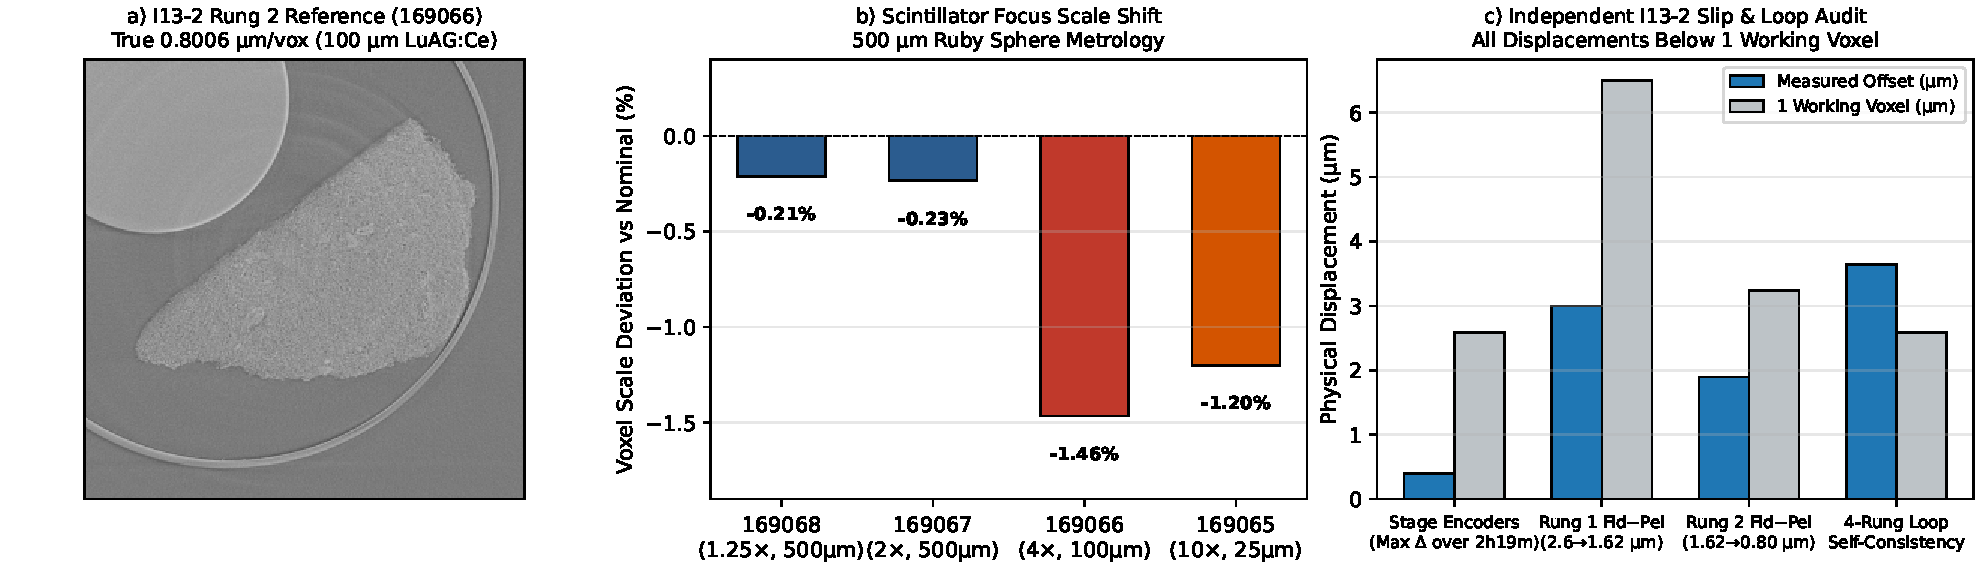
\includegraphics[width=\textwidth]{figures/fig1_metrology_and_ladder.pdf}
  \caption{I13-2 multi-magnification XCT metrology and stability audit: (a) \texttt{169066} mid-slice ($0.8006$\,\textmu m/vox); (b) ruby-sphere voxel calibration revealing the $-1.47\%$ thin-scintillator focal shift on the $4\times$ turret; (c) stage-encoder, fiducial-versus-pellet, and 4-rung loop self-consistency displacements compared against 1 working voxel.}
  \label{fig:metrology}
\end{figure}

\subsection{DIAD XRD-CT Calibration, \texorpdfstring{$-47.5^\circ$}{-47.5 deg} Rotation Offset, and Pending SCARF Checks}
Re-auditing the Zenodo \texttt{13329639} DIAD XRD-CT sinograms and Zenodo \texttt{13329670} Rigaku Cu-$\mathrm{K\alpha}$ powder standards resolved four physical discrepancies that previously degraded phase separation and $25 \leftrightarrow 50$\,\textmu m alignment:
\begin{enumerate}
  \item \textbf{Continuum \& $\Delta q$ calibration:} Subtracting the borosilicate capillary + air scattering continuum and correcting a $-0.00125\,\text{\AA}^{-1}$ zero-point $q$-offset between laboratory Cu-$\mathrm{K\alpha}$ references and the DIAD Pilatus3X CdTe detector cleanly separates $\mathrm{Na\text{-}13X}$ and $\mathrm{Zn\text{-}13X}$ via non-negative least squares (NNLS), revealing a monotonic axial ion-exchange gradient ($99.1\% \to 62.4\% \to 25.2\% \to 9.6\%$ Zn across \texttt{43324}, \texttt{43322}, \texttt{43323}, \texttt{43325}; Figure~\ref{fig:xrdct_series}).
  \item \textbf{$0^\circ/360^\circ$ duplicate frame \& COR audit:} Scan \texttt{43322} contains 79 projections ($0^\circ$--$355.4^\circ$), whereas \texttt{43323}--\texttt{43325} and all $50$\,\textmu m scans contain 80/40 frames repeating $0^\circ$ and $360^\circ$; averaging the duplicate endpoint and applying conjugate sub-pixel center-of-rotation (COR $\approx 19.5$\,px) removes streak asymmetry.
  \item \textbf{$-47.5^\circ$ soft-motor zero shift on all $50$\,\textmu m scans:} Between \texttt{k11-43325} ($25$\,\textmu m, $\theta \in [0^\circ, 360^\circ]$) and \texttt{k11-43336} ($50$\,\textmu m, $\theta \in [-47.5^\circ, 312.5^\circ]$), \texttt{gts\_cs\_theta} was re-zeroed by $-47.5^\circ$ while the physical start angle remained unchanged (frame-0 sinogram $r = 0.9956$ between \texttt{43324} and \texttt{43345}). Correcting $+47.5^\circ$ restores spatial alignment across all four slices.
\end{enumerate}

\noindent\fcolorbox{pendingframe}{pendingbg}{%
  \parbox{0.97\textwidth}{\small
  \textbf{Pending SCARF / Diamond Execution (Not Marked Done Until Run):}
  \textbf{(1) Stage 0A-2:} Zenodo DAWN exports retain only \texttt{/processed} (\texttt{kb\_cs\_y = 1080}\,px). While correlation margins on \texttt{43322}$\to$\texttt{43395} ($z{=}14$, $\Delta r{=}0.018$), \texttt{43323}$\to$\texttt{43398} ($z{=}17$, $\Delta r{=}0.014$), and \texttt{43325}$\to$\texttt{43399} ($z{=}18$, $\Delta r{=}0.025$) are clear, \texttt{43324}$\to$\texttt{43345} ($z{=}9$) leads \texttt{43346} ($z{=}10$) by $\Delta r{=}0.0052$ and must be verified via \texttt{registration/diad\_stage\_z\_audit.py} on \texttt{/dls/k11/data/2024/mg32980-1/nexus}, alongside 2D handedness against \texttt{k11-43334} ($0.54$\,\textmu m XCT).
  \textbf{(2) Stage 0C:} Full 32-bit cross-beamline registration (\texttt{169067} $\leftrightarrow$ \texttt{k11-43334}) via \texttt{registration/cross\_beamline\_audit.py} is pending on SCARF/Hamilton; Task T3 and XCT-guided T2 baselines remain gated until Stage 0C completes.}%
}

\begin{figure}[t]
  \centering
  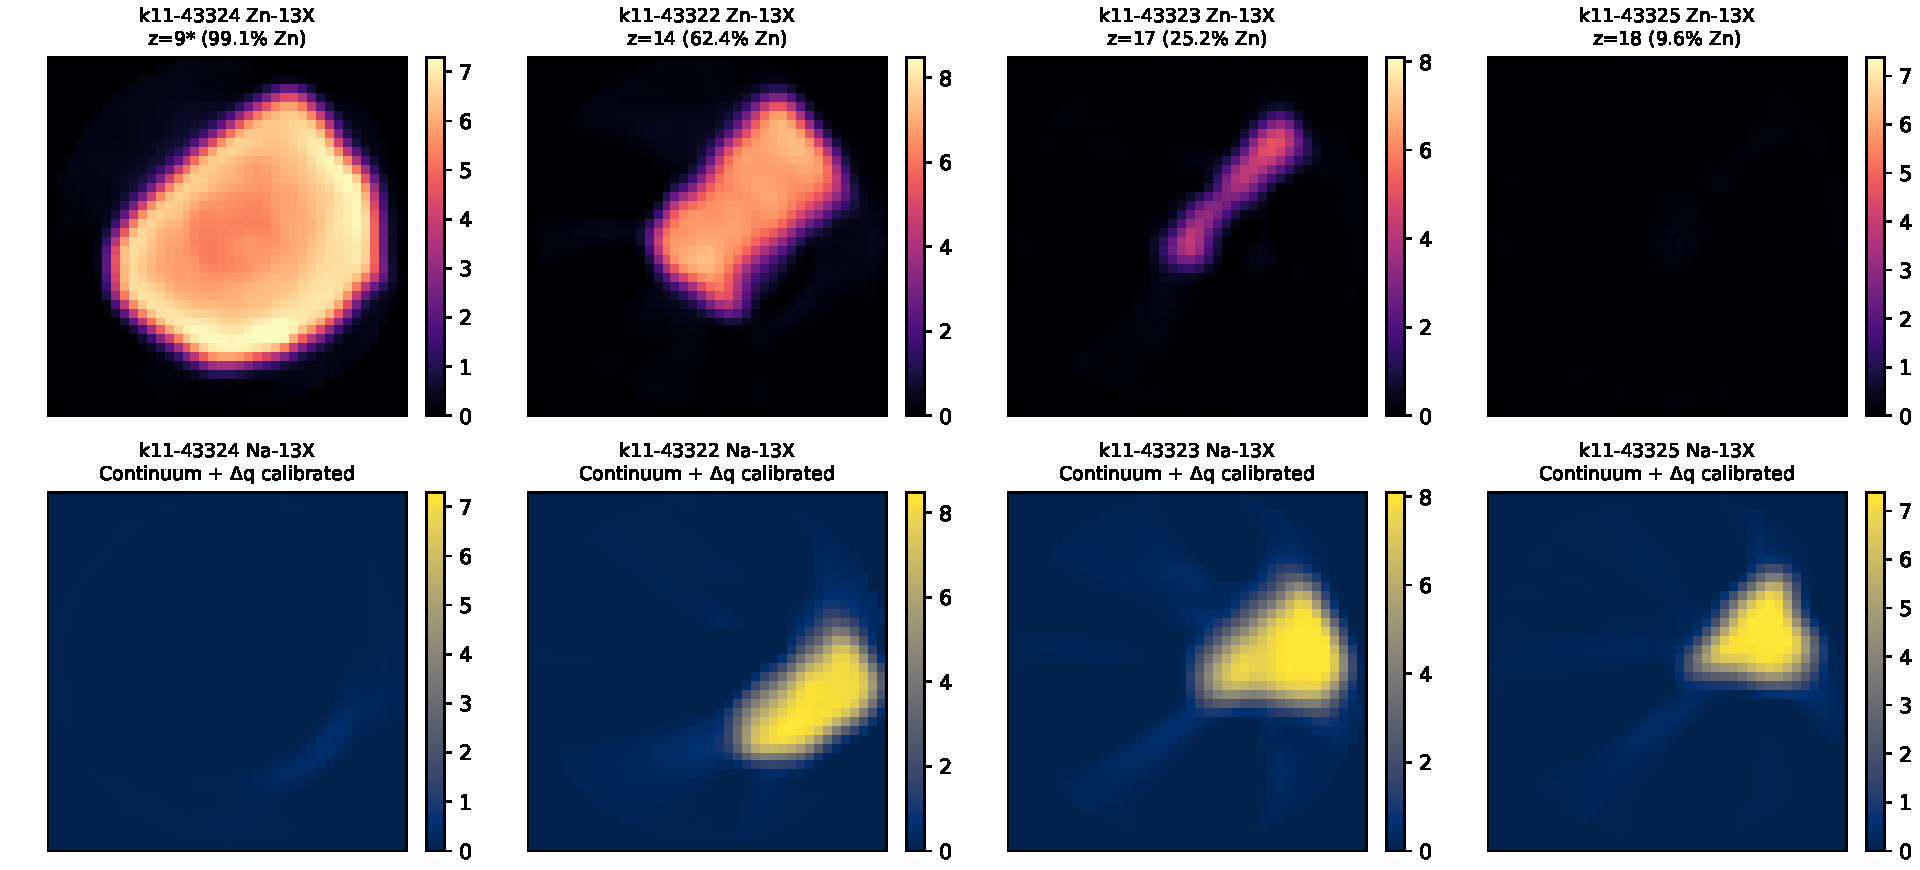
\includegraphics[width=\textwidth]{figures/fig2_xrdct_calibration_and_alignment.pdf}
  \caption{Continuum-subtracted and $\Delta q$-calibrated $25$\,\textmu m DIAD XRD-CT $\mathrm{Zn\text{-}13X}$ (top) and $\mathrm{Na\text{-}13X}$ (bottom) abundance maps across the four axial heights, resolving sharp core--shell reaction fronts on \texttt{43322} and \texttt{43323} ($^*$\texttt{43324} $z{=}9$ match pending Stage 0A-2 stage-$z$ confirmation).}
  \label{fig:xrdct_series}
\end{figure}

% =========================================================================
\section{Data Quality, Resolution Limits and Reference Tracks}
\label{sec:quality}
% =========================================================================

\paragraph{32-bit dynamic range and Fresnel fringes.}
Quantitative tasks exclusively use the 32-bit floating-point reconstructions (Zenodo \texttt{12206815}, \texttt{13327651}, \texttt{13327682}, \texttt{13327692}, \texttt{13349402}); the 8-bit sub-volumes (Zenodo \texttt{14245751}) clip high-attenuation ruby pixels and quantize zeolite contrast, so they are restricted to visual inspection. Because pink-beam propagation produces sharper Fresnel phase-contrast fringes at finer pixel sizes, T1 reports standard PSNR alongside Fresnel fringe-masked PSNR and band-limited PSNR.

\paragraph{True spatial resolution of $25$\,\textmu m vs.\ $50$\,\textmu m XRD-CT.}
We refer to the $25$\,\textmu m NNLS maps strictly as \emph{$25$\,\textmu m reference maps} rather than ``ground truth'', because $40 \times 79$ pencil-beam sinograms have finite angular sampling and noise. Splitting odd and even projections on continuum-subtracted reconstructions without hard-circle mask inflation (\texttt{circle=False}) yields raw half-data $\mathrm{FRC}(0.5) = 0.389$\,cyc/px ($64.3$\,\textmu m). Applying the Spearman--Brown full-dataset correction $\mathrm{FRC}_{\mathrm{full}} = 2\,\mathrm{FRC}_{1/2}/(1 + \mathrm{FRC}_{1/2})$ and van Heel's $1/2$-bit threshold~\cite{vanheel2005fourier} gives a true $25$\,\textmu m reference resolution of \textbf{$58.5$\,\textmu m} ($\mathrm{SB}_{0.5}$, $k = 0.43$\,cyc/px) and \textbf{$57.9$\,\textmu m} ($1/2$-bit), compared with \textbf{$103.6$\,\textmu m} ($\mathrm{SB}_{0.5}$) and \textbf{$111.5$\,\textmu m} ($1/2$-bit) on the matched $50$\,\textmu m maps---a true spatial resolution gain of \textbf{$1.79\times$--$1.93\times$} (Table~\ref{tab:frc}, Figure~\ref{fig:quality}a). All primary T2 error metrics are therefore band-limited to $k \le 0.43$\,cyc/px so models are never rewarded for fitting high-frequency reconstruction streaks.

\begin{table}[t]
\centering
\caption{Measured spatial resolution of $25$\,\textmu m reference vs.\ $50$\,\textmu m input DIAD XRD-CT maps ($n{=}4$ paired heights).}
\label{tab:frc}
\footnotesize
\begin{tabular}{lccc}
\toprule
Resolution Criterion (\texttt{circle=False} half-maps) & $25$\,\textmu m Reference & $50$\,\textmu m Input & True Resolution Ratio \\
\midrule
Raw Half-Split $\mathrm{FRC}(0.5)$ & $64.3$\,\textmu m ($0.389$\,cyc/px) & $120.1$\,\textmu m ($0.427$\,cyc/px) & $1.87\times$ \\
Spearman--Brown Full-Data $\mathrm{FRC}_{\mathrm{SB}}(0.5)$ & $58.5$\,\textmu m ($0.427$\,cyc/px) & $103.6$\,\textmu m ($0.496$\,cyc/px) & $\mathbf{1.79\times}$ \\
van Heel $1/2$-Bit Threshold~\cite{vanheel2005fourier} & $57.9$\,\textmu m ($0.432$\,cyc/px) & $111.5$\,\textmu m ($0.461$\,cyc/px) & $\mathbf{1.93\times}$ \\
\bottomrule
\end{tabular}
\end{table}

\paragraph{Why radial cupping detrending was rejected, and the Two-Track release.}
In partially exchanged Zeolite 13X, $\mathrm{Zn^{2+}}$ ($Z{=}30$) attenuates X-rays more strongly than $\mathrm{Na^+}$ ($Z{=}11$), creating both an axial attenuation trend and a radial core--shell profile inside each slice. Comparing candidate XCT cleanup fields directly against the $25$\,\textmu m $\mathrm{Zn\text{-}13X}$ XRD-CT maps proves that 7-term radial polynomial cupping detrending correlates strongly with real core--shell chemistry ($r = +0.281$ on \texttt{43322}, $r = +0.589$ on \texttt{43323}) and inverts radial intensity slopes by $-44.9\%$ on a synthetic ground-truth core--shell phantom, whereas conservative polar de-ringing is chemically uncorrelated ($|r| \le 0.026$) and retains $98.7\%$--$99.2\%$ of true pore-edge gradients (Figure~\ref{fig:quality}b,c). Zn-13X-Bench therefore publishes two reference tracks: \textbf{Primary (\texttt{raw\_float32})}, containing registered, uncleaned 32-bit float volumes; and \textbf{Secondary (\texttt{cleaned\_dering\_v1})}, applying only frozen conservative polar de-ringing, ruby-shadow $z$-masking, and XRD-CT $360^\circ$/COR fixes, accompanied by exact voxelwise difference maps.

\begin{figure}[t]
  \centering
  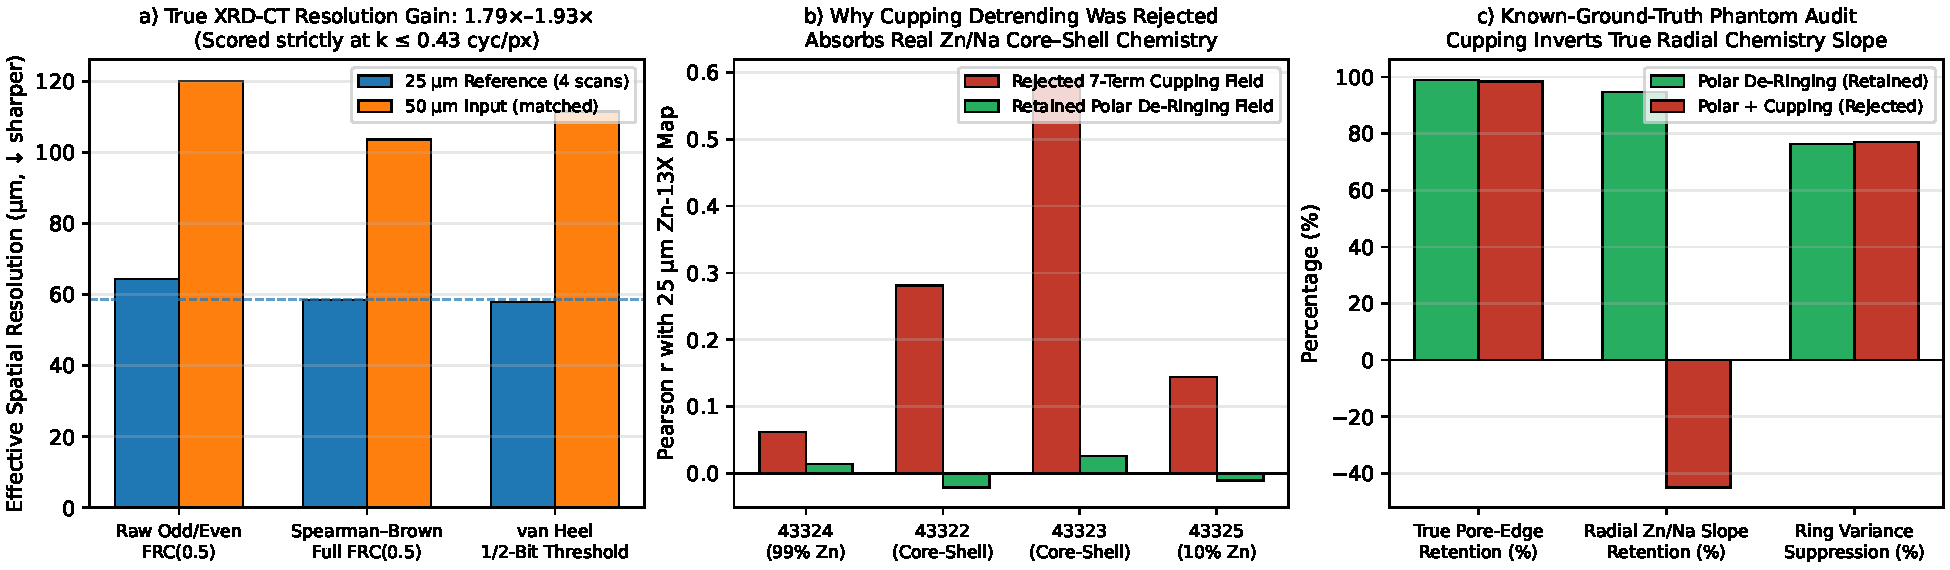
\includegraphics[width=\textwidth]{figures/fig3_frc_and_cupping_audit.pdf}
  \caption{Resolution limits and preprocessing audit: (a) XRD-CT effective spatial resolution across three FRC criteria ($1.79\times$--$1.93\times$ gain); (b) correlation of candidate XCT cleanup fields with real $25$\,\textmu m $\mathrm{Zn\text{-}13X}$ maps showing cupping detrending strips real chemistry; (c) synthetic phantom verification.}
  \label{fig:quality}
\end{figure}

% =========================================================================
\section{Tasks, Splits and Scoring}
\label{sec:tasks}
% =========================================================================

Zn-13X-Bench defines three core tasks (\textbf{T1--T3}) and one optional reconstruction extension (\textbf{T4}), summarized in Table~\ref{tab:tasks}. Artifact removal and standalone heuristic segmentation are intentionally excluded as benchmark tasks; segmentation enters strictly through a single fixed-threshold rule inside T1's \texttt{OpenImpala} transport scorer.

\begin{table}[t]
\centering
\caption{Summary of Zn-13X-Bench core tasks (\textbf{T1--T3}) and optional extension (\textbf{T4}).}
\label{tab:tasks}
\footnotesize
\begin{tabular}{lp{3.4cm}p{3.1cm}p{4.8cm}}
\toprule
Task & Input $\to$ Target & Baselines & Primary Scoring Metrics \\
\midrule
\textbf{T1}: Real-Pair XCT SR & Lower-res I13-2 \texttt{float32} rung $\to$ higher-res rung ($1.604\times$--$8.101\times$, frozen 7-DOF) & Tricubic, 3D U-Net, SwinIR~\cite{liang2021swinir}, OpenLSR-X & PSNR, fringe-masked PSNR, SSIM, 3D FSC; \texttt{OpenImpala} $|{\Delta D_{\mathrm{eff}}}|/D_{\mathrm{eff}}$, $|{\Delta\tau}|/\tau$, SSA, $\Delta\varepsilon$ + $\pm 5\%$ threshold sensitivity \\
\addlinespace[3pt]
\textbf{T2}: Chemical SR \& Fusion & $50$\,\textmu m XRD-CT Na/Zn ($+47.5^\circ$) + $0.54$\,\textmu m XCT$^\dagger$ $\to$ $25$\,\textmu m XRD-CT (4-fold LOSO) & Bicubic, Guided Filter~\cite{he2013guided}, Dual-Encoder U-Net, X-FUSE & Band-limited $\chi^2_\nu$ \& RMSE ($k \le 0.43$\,cyc/px), in-pellet $\mathrm{Na/Zn}$ corr.\ error, reaction-front pos.\ error (\textmu m) \\
\addlinespace[3pt]
\textbf{T3}: Cross-Beamline Reg.$^\dagger$ & Unaligned I13-2 (\texttt{169067}) \& DIAD (\texttt{k11-43334}) \texttt{float32} XCT $\to$ 7-DOF transform & 3-DOF Rigid, 7-DOF NMI, VoxelMorph~\cite{balakrishnan2019voxelmorph} & Fiducial / landmark TRE (mean, P95 \textmu m), scale error (\%), 8-octant residual drift (\textmu m) \\
\addlinespace[3pt]
\textbf{T4}: Sparse XRD-CT \emph{(Opt.)} & Subsampled $25$\,\textmu m sinograms (10, 20, 40 / 79 views) $\to$ full $79$-view recon & FBP (Hann), Non-Neg.\ SIRT, U-Net Post-Proc. & Noise-normalized $\chi^2_\nu$, RMSE, 2D $\mathrm{FRC}(0.5)$ \& $\mathrm{FRC}_{\mathrm{SB}}(0.5)$ \\
\bottomrule
\multicolumn{4}{l}{\scriptsize $^\dagger$XCT-guided T2 baselines and Task T3 are gated until Stage 0C cross-beamline registration runs on SCARF/Hamilton.}
\end{tabular}
\end{table}

\paragraph{Leakage-free splits in low-resolution voxels.}
A fixed physical buffer of $20$\,\textmu m spans fewer than 8 voxels at $2.6$\,\textmu m, allowing 3D patches and receptive fields to overlap across splits. In \texttt{splits/generate\_splits.py}, T1 axial slab buffers are therefore enforced in \emph{low-resolution voxels} ($\mathrm{patch\_z\_lr} + \mathrm{receptive\_field\_lr}$): $32 + 16 = 48$ LR voxels ($77.8$\,\textmu m) on the $2.026\times$ track and anisotropic $24 + 16 = 40$ LR voxels ($103.8$\,\textmu m, fitting cleanly within the 266 LR axial slices spanning \texttt{169065}) on the $8.101\times$ track, starting strictly above the 500\,\textmu m ruby sphere's pink-beam shadow ($z_0 \ge 640$ in \texttt{169066}). Because $\mathrm{Zn \to Na}$ exchange varies axially along the pellet, train/val/test slabs deliberately induce a documented out-of-distribution contrast shift. Task T2 uses 4-fold leave-one-slice-out (LOSO) cross-validation across \texttt{43324}, \texttt{43322}, \texttt{43323}, and \texttt{43325}, excluding $50$\,\textmu m slices within $\pm 100$\,\textmu m of the held-out test height from self-supervised pretraining.

% =========================================================================
\section{Baselines and the Synthetic-versus-Real Experiment}
\label{sec:baselines}
% =========================================================================

\subsection{Headline Experiment Protocol (T1 Synthetic-Trained vs.\ Real-Trained SR)}
For the $2.026\times$ (\texttt{169067}$\to$\texttt{169066}) and $8.101\times$ (\texttt{169068}$\to$\texttt{169065}) tracks, each learned backbone (3D U-Net, 3D SwinIR, and \texttt{OpenLSR-X}) is trained across three random seeds ($\{42, 137, 2026\}$) under three training regimes generated by \texttt{openlsrx\_adapter.py}: (i) \texttt{synthetic\_clean} (HR blurred and downsampled at the exact non-integer magnification ratio), (ii) \texttt{synthetic\_noisy} (adding calibrated sCMOS Poisson--Gaussian noise), and (iii) \texttt{real\_paired} (measured LR scan resampled via the frozen benchmark 7-DOF transform), totaling 54 GPU runs (\texttt{scripts/slurm/02\_t1\_headline\_array.sh}). All models are evaluated exclusively on real paired test slabs under one fixed Otsu threshold calibrated on the HR reference plus $\pm 5\%$ dynamic-range threshold sensitivity (Table~\ref{tab:t1_placeholder}).

\begin{table}[t]
\centering
\caption{Task T1 Headline Experiment schema (32-bit \texttt{raw\_float32} primary track; mean $\pm$ std over 3 seeds). All 54 GPU runs are scheduled via \texttt{scripts/slurm/02\_t1\_headline\_array.sh} and left unpopulated until executed on SCARF/Hamilton.}
\label{tab:t1_placeholder}
\resizebox{\textwidth}{!}{%
\begin{tabular}{llccccc}
\toprule
Track & Method \& Training Regime & PSNR (dB) $\uparrow$ & Fringe PSNR $\uparrow$ & FSC$_{0.5}$ $\uparrow$ & $|{\Delta D_{\mathrm{eff}}}|/D_{\mathrm{eff}}$ $\downarrow$ & $|{\Delta\tau}|/\tau$ $\downarrow$ \\
\midrule
$2.026\times$ & Tricubic (analytical) & \multicolumn{5}{c}{\pendingtag{Full 32-bit float32 slab extraction on SCARF}} \\
$2.026\times$ & 3D U-Net / SwinIR / OpenLSR-X (\texttt{synth\_clean}) & \multicolumn{5}{c}{\pendingtag{54-task SLURM GPU array}} \\
$2.026\times$ & 3D U-Net / SwinIR / OpenLSR-X (\texttt{synth\_noisy}) & \multicolumn{5}{c}{\pendingtag{54-task SLURM GPU array}} \\
$2.026\times$ & 3D U-Net / SwinIR / OpenLSR-X (\texttt{real\_paired}) & \multicolumn{5}{c}{\pendingtag{54-task SLURM GPU array}} \\
\midrule
$8.101\times$ & All regimes (chained adjacent 7-DOF) & \multicolumn{5}{c}{\pendingtag{54-task SLURM GPU array}} \\
\bottomrule
\end{tabular}%
}
\end{table}

\subsection{Executed XRD-CT Baselines on Real 32-bit Sinograms (Task T2 \& Optional Task T4)}
Because the full 32-bit DIAD XRD-CT sinograms (Zenodo \texttt{13329639}) are compact ($3.8$\,GB total), we executed the unguided 4-fold LOSO classical baselines for Task T2 and the sparse-view classical baselines for Optional Task T4 directly via \texttt{baselines/run\_xrdct\_classical\_suite.py} (Tables~\ref{tab:t2_results}--\ref{tab:t4_results}, Figure~\ref{fig:xrdct_baselines}).

In Task T2 (Table~\ref{tab:t2_results}), scalar beam-flux normalization $\alpha_{\mathrm{fold}}$ is fitted strictly on the three training slice pairs of each LOSO fold. While Bicubic improves full-band RMSE ($0.434$ vs.\ $0.446$), in-pellet $\mathrm{Na/Zn}$ correlation error ($0.562$ vs.\ $0.592$), and reaction-front localization ($15.30$\,\textmu m vs.\ $15.95$\,\textmu m) over Nearest interpolation on the three clear-margin slices, \emph{all unguided interpolators remain limited to $\sim 15.3$\,\textmu m reaction-front error and $\chi^2_\nu \approx 415$--$510$}, leaving a pronounced positive residual halo around the exterior pellet boundary (Figure~\ref{fig:xrdct_baselines}d) because $50$\,\textmu m chemical maps cannot sharpen macropore or exterior boundaries without high-resolution XCT structural guidance. On provisional slice \texttt{43324}, matching against \texttt{43345} ($z{=}9$) yields $37\%$ lower band-limited RMSE ($0.380$ vs.\ $0.600$) and $4.7\times$ lower $\chi^2_\nu$ ($631$ vs.\ $2992$) than \texttt{43346} ($z{=}10$).

In Optional Task T4 (Table~\ref{tab:t4_results}, Figure~\ref{fig:xrdct_baselines}e--h), evaluating across all four $25$\,\textmu m scans and both phases reveals a clear physical regime crossover: at $8\times$ angular undersampling (10/79 views), non-negative SIRT cuts FBP's streak-dominated RMSE by \textbf{47.2\%} ($0.237$ vs.\ $0.449$, $\chi^2_\nu = 236$ vs.\ $510$), whereas at $2\times$ undersampling (40/79 views), Hann-filtered FBP reaches $\chi^2_\nu = 0.58 < 1.0$ ($\mathrm{RMSE} = 0.060$, $\mathrm{FRC}_{\mathrm{SB}}(0.5) = 0.497$\,cyc/px), outperforming 60-iteration Landweber SIRT whose unweighted gradient steps converge slowly at high spatial frequencies.

\begin{table}[t]
\centering
\caption{Executed Task T2 4-fold LOSO classical baselines on real 32-bit DIAD XRD-CT maps ($k \le 0.43$\,cyc/px cut-off). We report both the 3 confirmed-margin slices (\texttt{43322}, \texttt{43323}, \texttt{43325}) and the 4-slice mean including provisional \texttt{43324}.}
\label{tab:t2_results}
\resizebox{\textwidth}{!}{%
\begin{tabular}{lcccc}
\toprule
Method (4-Fold LOSO) & Band-Lim.\ RMSE $\downarrow$ & Band-Lim.\ $\chi^2_\nu$ $\downarrow$ & $|\Delta r_{\mathrm{Na,Zn}}|$ $\downarrow$ & Front Pos.\ Err.\ (\textmu m) $\downarrow$ \\
 & 3-Conf.\ / All-4$^*$ & 3-Conf.\ / All-4$^*$ & 3-Conf.\ / All-4$^*$ & 3-Conf.\ / All-4$^*$ \\
\midrule
Nearest ($50 \to 25$\,\textmu m) & $0.4136$ / $0.4057$ & $415.2$ / $482.7$ & $0.5915$ / $0.5116$ & $15.95$ / $11.97$ \\
Bilinear ($50 \to 25$\,\textmu m) & $0.4525$ / $0.4387$ & $509.9$ / $554.7$ & $0.5756$ / $0.4972$ & $15.98$ / $12.01$ \\
Bicubic ($50 \to 25$\,\textmu m) & $0.4336$ / $0.4201$ & $476.0$ / $514.9$ & $\mathbf{0.5616}$ / $\mathbf{0.4855}$ & $\mathbf{15.30}$ / $\mathbf{11.49}$ \\
\midrule
Guided Filter / Dual U-Net / X-FUSE & \multicolumn{4}{c}{\pendingtag{Gated on Stage 0C DIAD $0.54$\,\textmu m XCT alignment}} \\
\bottomrule
\end{tabular}%
}
\end{table}

\begin{table}[t]
\centering
\caption{Executed Optional Task T4 sparse-view $25$\,\textmu m XRD-CT reconstruction baselines across all 4 scans $\times$ 2 phases (mean $\pm$ std vs.\ full 79-projection reference).}
\label{tab:t4_results}
\resizebox{\textwidth}{!}{%
\begin{tabular}{llcccc}
\toprule
Subsampled Views & Method & RMSE $\downarrow$ & Reduced $\chi^2_\nu$ $\downarrow$ & $\mathrm{FRC}(0.5)$ (cyc/px) $\uparrow$ & $\mathrm{FRC}_{\mathrm{SB}}(0.5)$ (cyc/px) $\uparrow$ \\
\midrule
10 / 79 ($\sim 8\times$) & FBP (Hann) & $0.4485 \pm 0.2584$ & $510.0 \pm 294.7$ & $0.2476 \pm 0.0258$ & $0.3300 \pm 0.0365$ \\
10 / 79 ($\sim 8\times$) & Non-Neg.\ SIRT & $\mathbf{0.2370 \pm 0.1456}$ & $\mathbf{236.1 \pm 167.2}$ & $\mathbf{0.2611 \pm 0.0448}$ & $0.3130 \pm 0.0459$ \\
\midrule
20 / 79 ($\sim 4\times$) & FBP (Hann) & $\mathbf{0.1485 \pm 0.0886}$ & $\mathbf{60.4 \pm 36.7}$ & $\mathbf{0.3924 \pm 0.0226}$ & $\mathbf{0.4393 \pm 0.0176}$ \\
20 / 79 ($\sim 4\times$) & Non-Neg.\ SIRT & $0.1950 \pm 0.1235$ & $169.6 \pm 133.9$ & $0.3487 \pm 0.0680$ & $0.3864 \pm 0.0659$ \\
\midrule
40 / 79 ($\sim 2\times$) & FBP (Hann) & $\mathbf{0.0604 \pm 0.0450}$ & $\mathbf{0.58 \pm 0.42}$ & $\mathbf{0.4913 \pm 0.0085}$ & $\mathbf{0.4965 \pm 0.0035}$ \\
40 / 79 ($\sim 2\times$) & Non-Neg.\ SIRT & $0.1874 \pm 0.1197$ & $155.1 \pm 127.1$ & $0.3753 \pm 0.0728$ & $0.3990 \pm 0.0706$ \\
\bottomrule
\end{tabular}%
}
\end{table}

\begin{figure}[t]
  \centering
  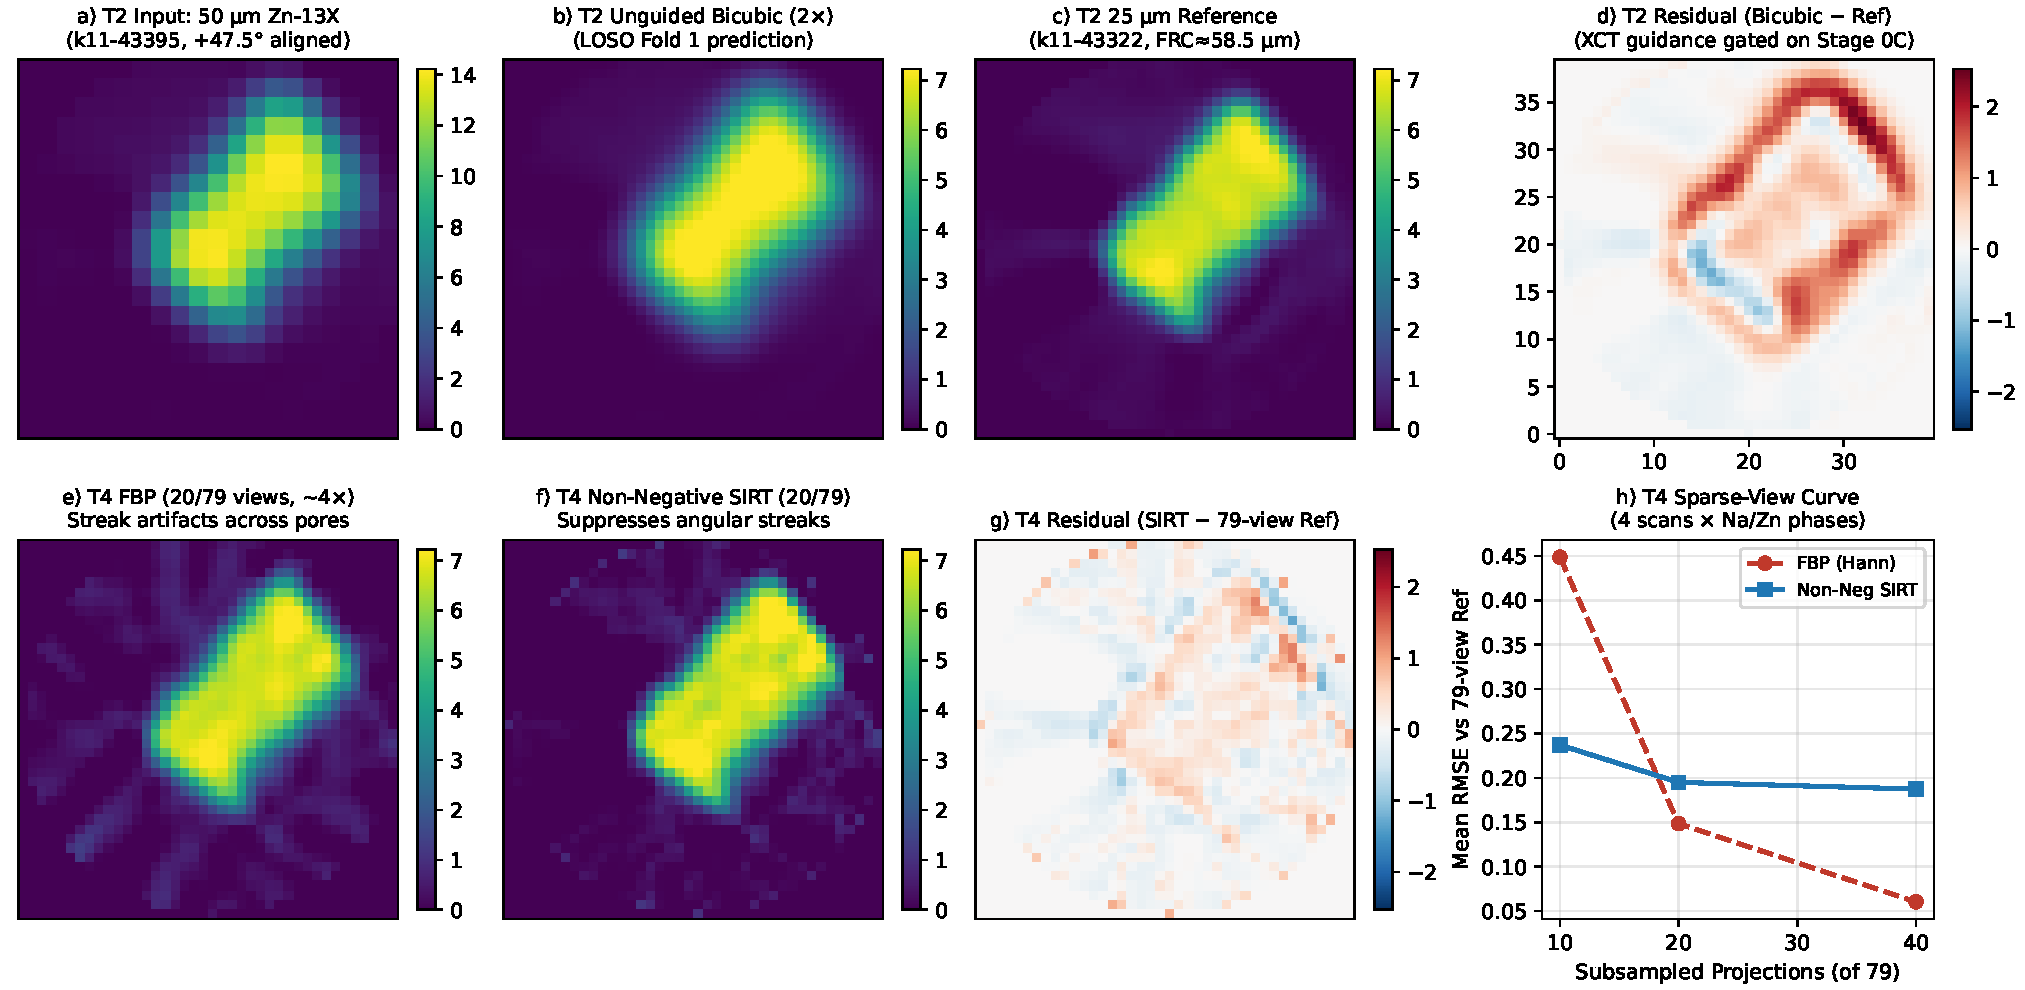
\includegraphics[width=\textwidth]{figures/fig4_xrdct_t2_t4_baselines.pdf}
  \caption{Executed real-sinogram baselines for Task T2 and Optional Task T4 on \texttt{k11-43322}: (a--d) unguided T2 Bicubic upsampling leaves a prominent outer-rim residual halo motivating XCT structural guidance; (e--h) T4 sparse-view reconstruction showing non-negative SIRT suppressing 10--20 view angular streaks while Hann FBP converges below the noise floor at 40 views.}
  \label{fig:xrdct_baselines}
\end{figure}

% =========================================================================
\section{Access, Format and Maintenance}
\label{sec:access}
% =========================================================================

Following NeurIPS Datasets and Benchmarks requirements, raw projections and full 53--57\,GB reconstructions remain permanently archived on their upstream CC-BY-4.0 Zenodo records~\cite{green2025synchrotron}. Our packaging pipeline (\texttt{release\_packaging/build\_derived\_release.py}) generates a derived Zenodo release linked via \texttt{isDerivedFrom} identifiers containing: (1) multiscale OME-Zarr v0.4~\cite{moore2021omenext} stores with physical \texttt{micrometer} coordinate transformations for both \texttt{raw\_float32} and \texttt{cleaned\_dering\_v1} tracks plus calibrated $25/50$\,\textmu m XRD-CT bundles; (2) frozen 7-DOF similarity transforms and leakage-free split manifests; (3) a $< 2$\,GB \texttt{zn13x\_bench\_lite} subset mirrored to Hugging Face Hub for rapid prototyping and CI; (4) validated MLCommons Croissant 1.0 metadata~\cite{akhtar2024croissant} (\texttt{configs/croissant.json}); and (5) a Gebru \emph{et al.}~\cite{gebru2021datasheets} Datasheet (\texttt{DATASHEET.md}). All metrics run deterministically via \texttt{python evaluate.py --task \{t1,t2,t3,t4\}}.

% =========================================================================
\section{Limitations}
\label{sec:limitations}
% =========================================================================

Four limitations govern interpretation of Zn-13X-Bench results:
(1) \textbf{Single specimen and material system:} All scans image one binderless Zeolite 13X pellet undergoing $\mathrm{Zn^{2+}/Na^+}$ exchange; generalization across rock, battery, or biological microstructures requires complementary multi-specimen benchmarks such as VoDaSuRe~\cite{vodasure2026}.
(2) \textbf{Axial chemistry shift across splits:} Disjoint axial T1 slabs sample different $\mathrm{Zn/Na}$ exchange fractions ($99\% \to 10\%$ Zn), coupling super-resolution evaluation with mild out-of-distribution contrast generalization.
(3) \textbf{Finite $25$\,\textmu m chemical resolution:} Because the $25$\,\textmu m XRD-CT reference resolves $\sim 58.5$\,\textmu m ($\mathrm{FRC}_{\mathrm{SB}}(0.5)$), T2 evaluates $1.79\times$--$1.93\times$ effective chemical sharpening up to $k = 0.43$\,cyc/px rather than sub-macropore resolution; predictions at $0.54$\,\textmu m XCT resolution are diagnostic only.
(4) \textbf{Threshold dependence of image-based PDE transport:} Continuous grayscale SR predictions must be binarized before \texttt{OpenImpala} Laplacian solves; applying one fixed reference-calibrated Otsu threshold alongside $\pm 5\%$ threshold sensitivity bounds---but does not eliminate---segmentation coupling.

\bibliographystyle{unsrt}
\bibliography{references}

\end{document}
